\newpage

\section{Supplementary material}
\label{sec:supp}

% \subsection{Detailed results for the letter arithmetic task}

%Table \ref{tab:results-t1} shows exact numbers for the simulations: Statistics for the learning time, the required teaching phases and the percentage of failures.

\begin{table}[h]
\centering
\small
\begin{tabular}{ll|rr}
\hline
\textbf{Policy} & \textbf{Simulated}  & \multicolumn{2}{l}{\textbf{Time to mastery in s}} \\ 
               & \textbf{Learner}    &   Median  & Conf. Interval \\ 
\hline
\multirow{3}{*}{Random} & Memoryless            & 936.8 & [751.8 976.6] \\
                        & Memory                & 110.5 & [102.0 125.4] \\
                        & Continuous            &  68.9 & [61.6 71.6]   \\
\hline
\multirow{3}{*}{Random  QE only} & Memoryless   & 814.4 & [814.0 815.2] \\
                        & Memory                & 102.2 & [82.0 121.6]  \\
                        & Continuous            &  80.8 & [61.4 81.2]   \\
\hline
\multirow{3}{*}{\makecell[l]{Max. Info. \\ Gain}}
                        & Memoryless            & 462.0 & [346.5 535.5] \\
                                & Memory        &  42.0   & [42.0 42.0]   \\
                                & Continuous    &  42.0   & [42.0 42.0]   \\
\hline
\hline
\multirow{3}{*}{Memoryless}     & Memoryless    & 313.2 & [271.0 396.2] \\
                                & Memory        &  62.6 & [42.0 62.6]   \\
                                & Continuous    &  42.0   & [42.0 42.0]   \\
\hline
\multirow{3}{*}{Memory}       & Memoryless      & 466.1 & [311.4 517.0] \\
                                & Memory        &  42.0   & [42.0 42.0]   \\
                                & Continuous    &  42.0   & [42.0 42.0]   \\
\hline
\multirow{3}{*}{Continuous}     & Memoryless    & 794.8 & [794.8 794.8] \\
                                & Memory        &  42.0   & [21.0 42.0]   \\
                                & Continuous    &  42.0   & [42.0 42.0]   \\

\hline
\end{tabular}
\caption{Results for the \textit{letter arithmetic} task for the different planning algorithms with corresponding learner models. Bootstrapped 68\% confidence intervals are reported in brackets.
% The original paper only reported median values. The learn time is calculated based on the provided costs for the different action types from the original paper. It does not include time needed for the assessment. Teaching phases consisted of 3 actions, maximum 40 phases were performed before termination. The failed rate shows the percentage of learners that did not learn the correct concept in these 40 phases.
}
\label{tab:results-t1}
\end{table}

\begin{table}[hb!]
\centering
\small
\begin{tabular}{ll|r|r|r}
\hline
\textbf{Policy} & \textbf{Sim.}  &  \multicolumn{1}{l|}{\textbf{Multiples of 7}}  & \multicolumn{1}{l|}{\textbf{Mult. of 4 minus 1}} &  \multicolumn{1}{l}{\textbf{Range 64-83}} \\
                    & \textbf{Learner}    & Time (MD [CI]) & Time (MD [CI]) & Time (MD [CI]) \\
\hline
\multirow{3}{*}{Random}                                         & Mless    & 	 224.80 [196.80 284.20] & 641.00 [538.10 656.10] & 98.60 [88.80 123.20]  \\
                                                                & Memory        & 	 33.40 [30.80 37.00]    & 166.20 [143.40 208.40] & 57.40 [49.60 67.70]   \\
                                                                & Cont.    & 	 32.00 [29.40 34.00]    & 51.60 [45.00 54.60]    & 42.00 [34.80 47.80]   \\
\hline
\multirow{3}{*}{\makecell[l]{Random \\ QE only}}                & Mless    & 	 130.20 [116.40 146.00] & 515.40 [428.00 516.80] & 77.80 [58.40 91.60]   \\
                                                                & Memory        & 	 38.40 [38.00 39.20]    & 91.40 [89.60 104.00]   & 58.60 [51.80 65.60]   \\
                                                                & Cont.    & 	 26.60 [26.00 32.80]    & 45.80 [39.60 52.00]    & 51.60 [50.40 52.40]   \\
\hline
\multirow{3}{*}{\makecell[l]{Maximum \\ Information \\ Gain}}   & Mless    & 	 168.00 [132.00 204.00] & 480.00 [480.00 480.00] & 108.00 [96.00 156.00] \\
                                                                & Memory        & 	 12.00 [12.00 12.00]    & 12.00 [12.00 12.00]    & 12.00 [12.00 12.00]   \\
                                                                & Cont.    & 	 12.00 [12.00 12.00]    & 12.00 [12.00 12.00]    & 12.00 [12.00 12.00]   \\
\hline\hline
\multirow{3}{*}{Memoryless}                                     & Mless    & 	 120.60 [96.80 140.20]  & 480.00 [480.00 480.00] & 60.00 [36.00 60.00]   \\
                                                                & Memory        & 	 12.00 [12.00 12.00]    & 48.00 [18.00 66.00]    & 24.00 [24.00 24.00]   \\
                                                                & Cont.    & 	 12.00 [12.00 12.00]    & 12.00 [12.00 12.00]    & 24.00 [24.00 24.00]   \\
\hline
\multirow{3}{*}{Memory}                                         & Mless    & 	 90.00 [72.00 108.00]   & 485.40 [485.00 487.20] & 24.00 [24.00 24.00]   \\
                                                                & Memory        & 	 12.00 [12.00 12.00]    & 41.60 [38.80 50.60]    & 24.00 [12.00 24.00]   \\
                                                                & Cont.    & 	 12.00 [12.00 12.00]    & 26.20 [26.00 26.40]    & 24.00 [24.00 24.00]   \\
\hline
\multirow{3}{*}{Continuous}                                     & Mless    & 	 192.00 [144.00 270.00] & 482.40 [482.40 482.40] & 94.00 [63.20 129.00]  \\
                                                                & Memory        & 	 12.00 [12.00 12.00]    & 230.40 [194.40 285.60] & 48.80 [38.00 56.60]   \\
                                                                & Cont.    & 	 12.00 [12.00 12.00]    & 26.40 [26.40 26.40]    & 24.40 [24.40 24.80]   \\

\hline
\end{tabular}
\caption{Time to mastery for the \textit{number game} tasks for each policy with corresponding learner models. Reported are medians and the bootstrapped 68\% confidence intervals (in brackets).
%The time is calculated based on the provided costs for the different action types from the original paper. It does not include time needed for the assessment. Teaching phases consisted of 3 actions, maximum 40 phases were performed before termination. The failed rate shows the percentage of learners that did not learn the correct concept in these 40 phases.
}
\label{tab:results-t2}
\end{table}


%%% Lukas: as this is only done in a naive way for the first task, I remove it in the end
% \subsection{Results for memoryless and discrete models with paired updates}

% Improving the original definitions for the memoryless and discrete models with paired updates improves the results. With this change, the memoryless model performs decent as well. Paired update refers to updating the hypothesis about the true concept based on the new evidence shown, and updating first one possible pair of letters which would fulfill the new evidence, after which the remaining letters are mapped randomly to result in a complete and unique mapping. This effectively prefers states that are close to the current state of the learner, implicitly keeping previously learned in the state.

% \begin{figure}
%     \centering
%     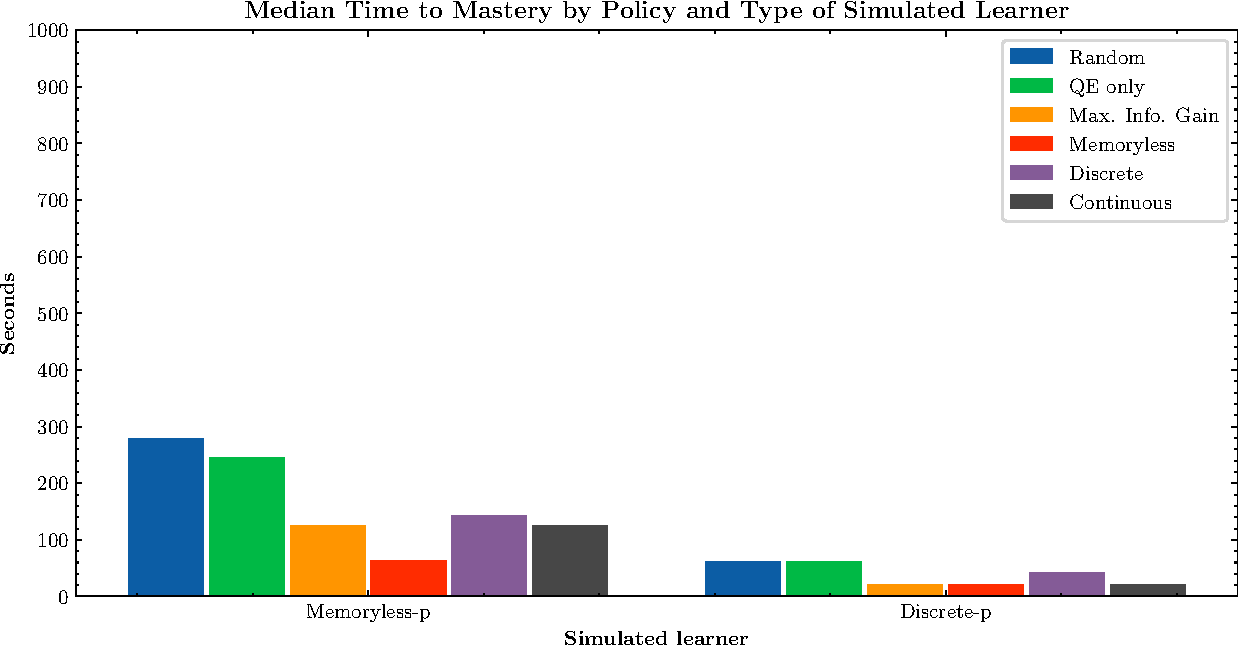
\includegraphics[width=\linewidth]{median-time-paired.pdf}
%     \caption{Planned action type per step for each planning model. Example actions were predominantly chosen. The memoryless model sometimes added }
%     \label{fig:md-time-paired}
% \end{figure}

% \begin{table}
% \centering
% \begin{tabular}{ll|rrr|rrr|r}
% \hline
% \textbf{Model} & \textbf{Simulated}  & \multicolumn{3}{l|}{\textbf{Learn time in s}}   & \multicolumn{3}{l|}{\textbf{Teaching phases}}   & \textbf{Failed} \\ 
%               & \textbf{Learner}    &   MD  & M     & SD                              & MD    & M     & SD                              &                 \\ 
% \hline
% \multirow{2}{*}{Random} & Memoryless-p         & 279.2 & 354.4 &  281.7               & 11.0  & 14.0  & 11.0                  &  2\%            \\
%                         & Discrete-p           &  61.3 &  82.7 &   72.3               &  2.5  &  3.3  &  2.7                  &  0\%            \\
% \hline
% \multirow{2}{*}{\makecell[l]{Random \\ QE only}} 
%                         & Memoryless-p          & 245.4 & 298.4 & 228.7             & 12.0 & 14.6 & 11.2                   &  6\%                \\
%                         & Discrete-p            &  61.4 & 81.8 &  59.5              &  3.0 &  4.0 &  2.9                   &  0\%                \\
% \hline
% \multirow{2}{*}{\makecell[l]{Maximum \\ Info. Gain}}   
%                                 & Memoryless-p  & 126.0 & 180.2 & 149.4               &  6.0 &  8.6 &  7.1                   &  0\%                \\
%                                 & Discrete-p    &  21.0 &  30.2 &  11.2               &  1.0 &  1.4 &  0.5                   &  0\%                \\
% \hline
% \hline
% \multirow{2}{*}{Memoryless}     & Memoryless-p  &  63.0 &  84.5 &  61.1               &  3.0 &  4.0 &  2.9                   &  0\%                \\
%                                 & Discrete-p    &  21.0 &  32.3 &  16.3               &  1.0 &  1.5 &  0.8                   &  0\%                \\
% \hline
% \multirow{2}{*}{Discrete}       & Memoryless-p  & 143.0 & 161.7 & 126.2               &  7.0 &  7.8 &  6.1                   &  0\%                \\
%                                 & Discrete-p    &  42.0 &  43.2 &  16.8               &  2.0 &  2.1 &  0.8                   &  0\%                \\
% \hline
% \multirow{2}{*}{Continuous}     & Memoryless-p  & 126.0 & 175.1 & 148.5               &  6.0 &  8.3 &  7.1                   &  0\%                \\ 
%                                 & Discrete-p    &  21.0 &  32.8 &  17.4               &  1.0 &  1.6 &  0.8                   &  0\%                \\

% \hline
% \end{tabular}
% \caption{Results for learners reducing state space distances between transitions (paired update mode). Only valid for memoryless and discrete learners. It is applied to the same stochastic planning models, which results in more conservative planning. The results might suggest that the assumptions about these two learner models were too simple to be usable. In paired mode, the memoryless model performs significantly better (even though it is not fully minimizing distances yet). The discrete memory paired version also performs better, even beating the continuous model slightly.}
% \label{tab:results-paired}
% \end{table}

%\subsection{Results: figures of means}

%This section contains additional figures using means and standard deviations for the simulation results.

%\begin{figure}
%    \centering
%    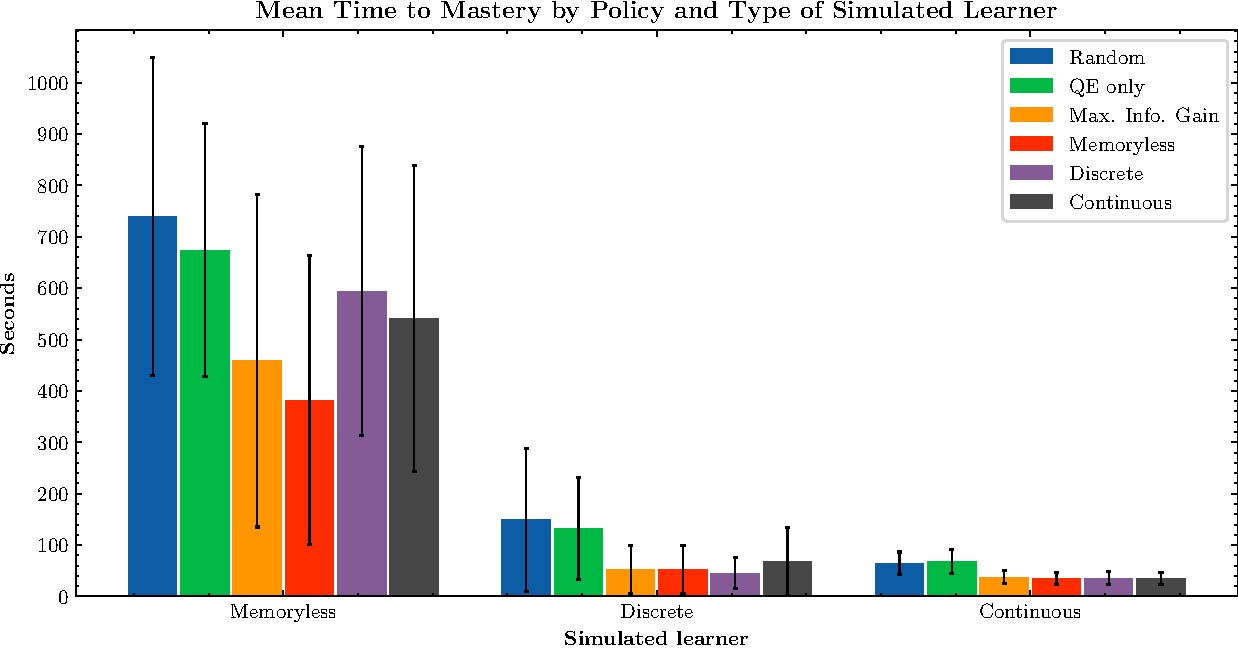
\includegraphics[width=\linewidth]{mean-time.pdf}
%    \caption{Mean time to mastery}
%    \label{fig:mean-time}
%\end{figure}

%\begin{figure}
%    \centering
%    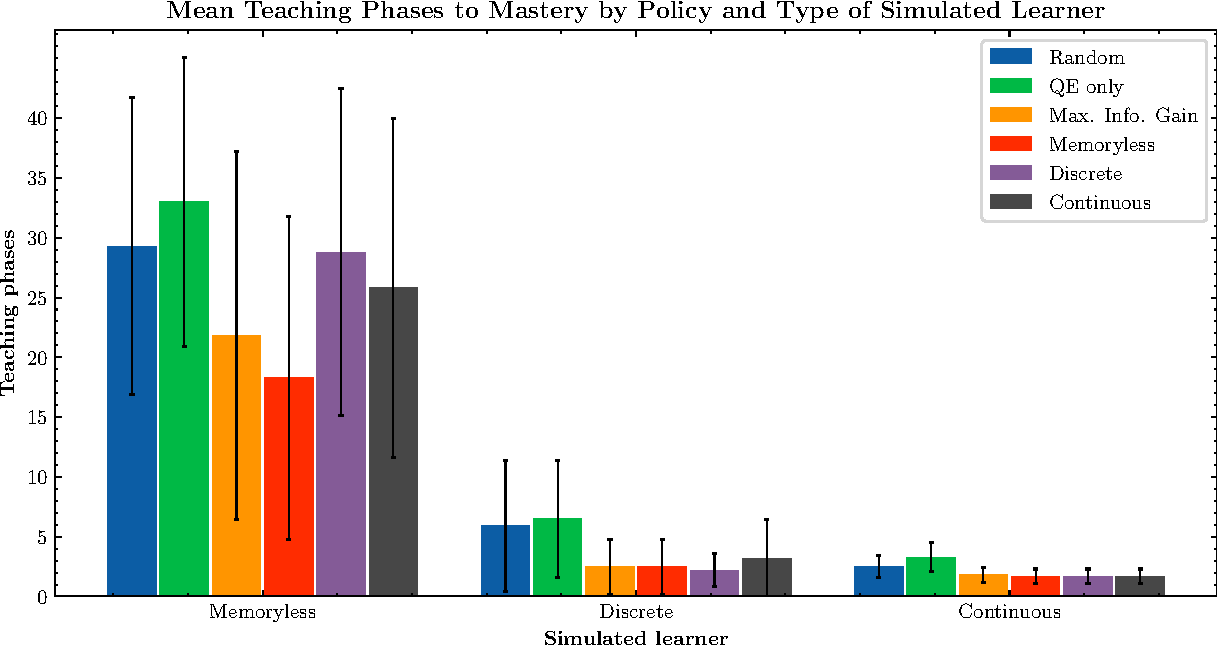
\includegraphics[width=\linewidth]{mean-phases.pdf}
%    \caption{Mean phases to mastery}
%    \label{fig:mean-phases}
%\end{figure}